\documentclass[12pt,a4paper]{article}
\usepackage[utf8]{inputenc}
\usepackage[english]{babel}
\usepackage{amsmath}
\usepackage{amsfonts}
\usepackage{amssymb}

\usepackage{graphicx}
\usepackage{subcaption}

\usepackage[left=2cm,right=2cm,top=2cm,bottom=2cm]{geometry}

\usepackage[]{algorithm}
\usepackage{algpseudocode}

\usepackage{placeins}	% Floatbarrier


\author{Elias Röger, Ekaterina Tikhoncheva}
\title{Force Directed Graph Drawing Algorithms}
\date{23.02.2015}



\begin{document}
\maketitle
%\tableofcontents    %inhaltszerzeichniss noetig ja nein?

\section{Introduction}

The drawing of graphs, that satisfy some predefined conditions, is one of the most important topics in different fields of application such as information visualisation or chips production. There are a lot of different techniques of drawing the \glqq nice\grqq\ graphs. In this work we present two algorithms from class of force-directed graph drawing algorithms \cite{Kobouro}. In the first section we consider the approach by T. Kamada and S. Kawai \cite{TomihisaKamada1989} from $1988$ and in the second section the multi-scale algorithm by D. Harel and Y. Koren \cite{DavidHarel2002}, which can be considered as extension of each force-directed graph drawing algorithm to deal with bigger graphs. In the last section we report the results of our implementations of both algorithms and compare them with the results from the papers.


\section{Algorithm by Kamada and Kawai}
\label{section1}

We implemented an algorithm for drawing general undirected graphs from \cite{TomihisaKamada1989}. In the following we refer to this algorithm as KKA (Kamda Kawai algorithm). \\ KKA visualizes connected, weighted, undirected graphs as a 2 dimensional picture where the edges are drawn as straight lines between the vertices. The authors state objectives for their graph drawing algorithm:
\begin{enumerate}
	\item uniform distribution of vertices and edges
	\item preserve symmetric structures
	\item low number of edge crossings
\end{enumerate}

The first two objectives are more important for human understanding than the third one. Hence, the goal of KKA is to find a state where the vertices and edges are distributed uniformly. 2. and 3. often follow from that. \\
We can now describe an optimal drawing of a graph mathematically. We try to minimize the sum of the differences between the desirable (Euclidian) distances and the actual distances between all pairs of vertices. Now let $G = (V,E)$ be a graph with $n = |V|$ vertices. We define $ p_1 , \dots, p_n$ as the projections into the 2 dimensional plane of the vertices $v_1, \dots , v_n \in V$ . The appropriate mapping $L:V\rightarrow\mathbb{R}^2$ is called a layout of a graph $G$. We now define the function
\begin{align}
\label{energyf}
E(p_1 , \dots, p_n) = \sum_{i=1}^{n-1} \sum_{j=i+1}^n \frac{1}{2} k_{ij} \lbrace | p_i - p_j | - l_{ij} \rbrace^2
\end{align}
which models the imbalance of our drawing. We define $(d_{ij})_{i,j = 1, \dots,n}$ as the matrix of distances between all vertices and $(l_{ij})_{i,j = 1, \dots,n} = L \times d $ is a scaled distance. $(k_{ij})_{i,j = 1, \dots,n}$ is a weight matrix and its entries are defined by $k_{ij} = K / d_{ij}^2$. Since our graphs are undirected $d, l$ and $k$ are symmetric. \\ 
We now try to find a local minimum of $E$. Consequently we are looking for $p_m$ with 
\begin{align*}
\frac{\partial E}{\partial p_m} = 0 \quad for \ m=1, \dots,n.
\end{align*}
This yields $2n$ nonlinear equations. We set $p_m = (x_m, y_m)$ and solve the equation for every $m$ by using the two-dimensional Newton-Raphson Method. The means we iterate
\begin{align*}
\begin{pmatrix}
x_m^{t+1} \\
y_m^{t+1}
\end{pmatrix}
=
\begin{pmatrix}
x_m^t + \delta x \\
y_m^t + \delta y
\end{pmatrix}.
\end{align*}
and stop when $\Delta_m := \sqrt{\frac{\partial E}{\partial x_m}^2 + \frac{\partial E}{\partial y_m}^2}$ is smaller than a predefined $ \epsilon$ for all $m$. 
The increments $\delta x$ and $\delta y$ are defined by
\begin{equation}
\label{NR_iteration}
\begin{aligned}
	\frac{\partial^2 E}{\partial x_m^2}(x_m^t,y_m^t) \delta x + \frac{\partial^2 E}{\partial x_m \partial y_m}(x_m^t,y_m^t) \delta y = - \frac{ \partial E}{\partial x_m} (x_m^t,y_m^t),\\	
	\frac{\partial^2 E}{\partial y_m \partial x_m}(x_m^t,y_m^t) \delta x + \frac{\partial^2 E}{\partial y_m^2}(x_m^t,y_m^t) \delta y = - \frac{ \partial E}{\partial y_m} (x_m^t,y_m^t).
\end{aligned}
\end{equation}

This leads to the algorithm:

\begin{algorithm}
\caption{Kamada Kawai \cite{TomihisaKamada1989}}
\label{KKA}
\begin{algorithmic}[1]
\item Compute the matrices d, l and k
\item initialize $p_1 , \dots, p_n$ 
\While {$( \max \Delta_i > \epsilon)$}
	\State $ m = argmax \Delta_i $
	\While {$\Delta_m > \epsilon$}
		\State compute $\delta x$ and $\delta y$
		\State iterate $x_m = x_m + \delta x$, $y_m = y_m + \delta y$
		\State compute $\Delta_m$
	\EndWhile
	\State compute $\Delta_i$ for $i=1, \dots, n$
\EndWhile
\end{algorithmic}

\end{algorithm}

\newpage

\section{A fast multi-scale algorithm by D. Harel and Y. Koren}
\label{section2}

The second algorithm we tested is the algorithm by D. Harel and Y. Koren \cite{DavidHarel2002} (further HKA), which also handle the problem of drawing an undirected graph $G=(V,E)$ with straight line edges.

The issue, the authors were dealing with, is the low speed of the most at the time force-directed drawing algorithms due to optimization of the quadratic energy function, which makes them almost inapplicable for the large graphs with more than $1000$ vertices. To cope with the speed problem authors continued the approach from \cite{HadanyHarel2001} and suggested new faster multi-scale algorithm.

The idea of the their algorithm is very simple: instead of consider the whole graph $G$ at ones one builds an approximation sequence of coarse graphs $G^{k_1}, G^{k_2}, \dots, G^{k_l},\ k_1<k_2<\dots<k_l=|V|$ ({\it multi-scale representation of G}), and applies one of the simple force-directed drawing algorithm to draw those graphs nicely. Beatification of each scale provides a locally nice layout of $G$ and sequence of all locally nice layouts approximates the nice layout of $G$. We refer to the paper \cite{DavidHarel2002} for theoretical background of multi-scale representation of a graph, locally and globally nice layouts and describe here only the algorithm presented by authors.

\subsubsection*{Algorithm}
To build a coarse graph of a given graph $G$ authors suggest to cluster vertices of $G$ in $k$ groups, so that the distance between vertices in the same group is minimized. This corresponds to the simple observation, that the vertices, which are close to each other according to graph distances, should also be drawn closer.

The algorithm \ref{kclusters} provides a simple heuristic approach for the $k$-clustering problem. In the new coarser graph the vertices in one cluster will be merged together in a single vertex - corresponding cluster center.

\begin{algorithm}
\caption{K-Centers($G(V,E),k$) \cite{DavidHarel2002}}
\label{kclusters}
\begin{algorithmic}[1]
\State $S=\{v\}$ for some arbitrary $v\in V$
\For {every $i = 2$ to $k$}
	\State find $u$ such that $min_{s\in S}d_{us}>min_{s\in S} d_{ws}\ \forall w\in V$ 
	\State $S = S\cup\{u\}$
\EndFor \\
\Return $S$
\end{algorithmic}
\end{algorithm}

For local layout beatification the algorithm of the Kamada and Kawai (see section \ref{section1}) with two small changes was selected. First, the algorithm is running predefined number of iterations without testing the condition in line $5$, see algorithm \ref{KKA}. Second change is, that we consider only $r$-neighbourhood of each vertex, where $r$-neighbourhood of a vertex v is defined as $N^r(v)=\{u\in V| 0\le d_{uv}<r\}$. That means, that formula (\ref{energyf}) in the modified version has the form:
\begin{align}
\label{energyf_HK}
E(p_1 , \dots, p_n) = \sum_{i\in V} \sum_{j\in N^r(i)} \frac{1}{2} k_{ij} \lbrace | p_i - p_j | - l_{ij} \rbrace^2
\end{align}

The described variation of the Kamada and Kawai algorithm is summarized in algorithm \ref{KKAmod}.

\begin{algorithm}
\caption{LocalLayoutG($d_{V\times V}$, $L$, $k$, $Iterations$) \cite{DavidHarel2002}}
\label{KKAmod}
\begin{algorithmic}[1]
\For {every $i = 1$ to $Iterations \cdot |V|$}
	\State $v = argmax_{u}\ \Delta^k_u$
	\State compute $\delta^k_v$ by solving equations (\ref{NR_iteration})
	\State $L(v)=L(v) + (\delta^k_v(x), \delta^k_v(y))$
\EndFor
\end{algorithmic}
\end{algorithm}

\FloatBarrier 

The complete algorithm of Harel and Koren is listed below:

\begin{algorithm}
\caption{LayoutG(V,E) \cite{DavidHarel2002}}
\label{HK}
\begin{algorithmic}[1]
\item Set constants $Rad$, $Iterations$, $Ratio$, $MinSize$
\item Compute the all-pairs shortest length $d_{V\times V}$
\item Set up random layout L
\State $ k = MinSize $
\While {$k\le |V|$}
	\State $ centers =  \mathbf{K-Centers(G(V,E),k)} $
	\State $ radius =  \max_{v\in centers}\min_{u\in centers}d_{vu} \cdot Rad $	
	\State $\mathbf{LocalLayout}(d_{centers\times centers}, L(centers), radius, Iterations)$
	\For {every $v\in V$}
		\State $L(v)=L(centers(v))+rand$
	\EndFor
	\State $k = k \cdot Ratio$
\EndWhile \\
\Return L
\end{algorithmic}
\end{algorithm}

Notice a random noise ($(0,0)<rand<(1,1)$) added at line $10$ to coordinates of vertices.
In the following section we represent the result of evaluation both algorithms in our implementation on the examples from corresponding papers.

\section{Implementation}
The both described algorithms were implemented with Python (version 2.7.6) and included in simple GUI for better visualisation proposes (see Fig. \ref{fig: 0}). The GUI was designed with QT Creator 3.2.2 and then bound with Python using PyQt version 4.11. The results of evaluation were obtained on two different laptops, but we mention by each table with performance results the hardware specification of the corresponding laptop.

\begin{figure}
	\centering
	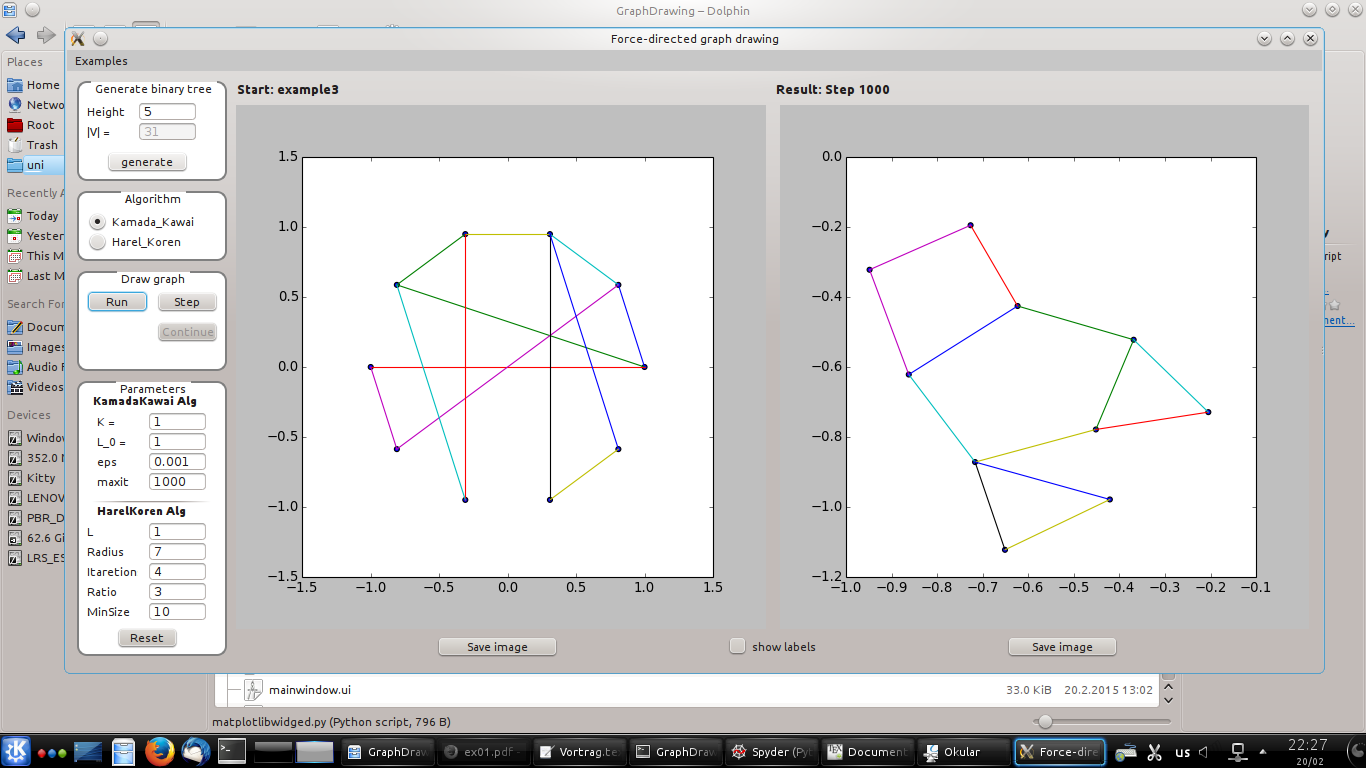
\includegraphics[scale=0.4]{interface.png}
	\caption{GUI}\label{fig: 0}
\end{figure}

In our code we used the following additional libraries : numpy (version 1.8.2) and scipy (version 0.13.3). Our implementation is unfortunately pure optimized, so that the better optimized version will probably perform better. But we did some optimization, because the initial implementation contained a lot of loops, which are rather slow in Python. So we used a vectorization to get rid of loops in the realisation of described algorithms.

It is also worth to mention that calculation of pairwise distance between all vertices of a given graph is extremely time consuming. In our implementation we first followed the idea in \cite{TomihisaKamada1989} and used Floyd's algorithm for shortest paths \cite{Floyd1962}. Since this has complexity $ O(|V|^3)$ we also implemented a version of Dijkstras algorithm. For graphs with more than 1000 vertices we decided to use a heavily optimized version of Dijkstras algorithm from the scipy library. In the both papers \cite{TomihisaKamada1989} and \cite{DavidHarel2002} this problem did not arise, because the first one considers the graphs with fewer vertices and in the second an additional library for efficient algorithm on graphs was used.

\section{Evaluation results}

As start layout we initialize vertices of the graph uniformly on a circle with radius $L_0$. That means viewed as complex variables we can write 
\begin{align*}
p_m =L_0 \times e^{2 pi*i*m /n}
\end{align*}
For some examples we load the initial positions of vertices from corresponding input file (example of the 3elt graph from Scotch collection \cite{JordiPetit})\\

We tested both algorithm with different graphs from \cite{TomihisaKamada1989} and \cite{DavidHarel2002}. 

\FloatBarrier 

\subsubsection*{Algorithm of Kamada and Kawai}

In figure \ref{fig: 1} we show the initial state of a graph, the first two steps \footnote{we refer to one iteration of the outer loop as one step}  and the state the graph converges to after 49 steps. In the first step the vertex $v_2$ gets moved to the middle. In the second step vertex $v_6$ gets moved. After this we already have a graph without edge crossing. In the following steps the movements are smaller and lead to a symmetric graph, where all the edges have the same length.

\FloatBarrier 

\begin{figure}
			\begin{minipage}[b]{.24\textwidth}
			\centering
			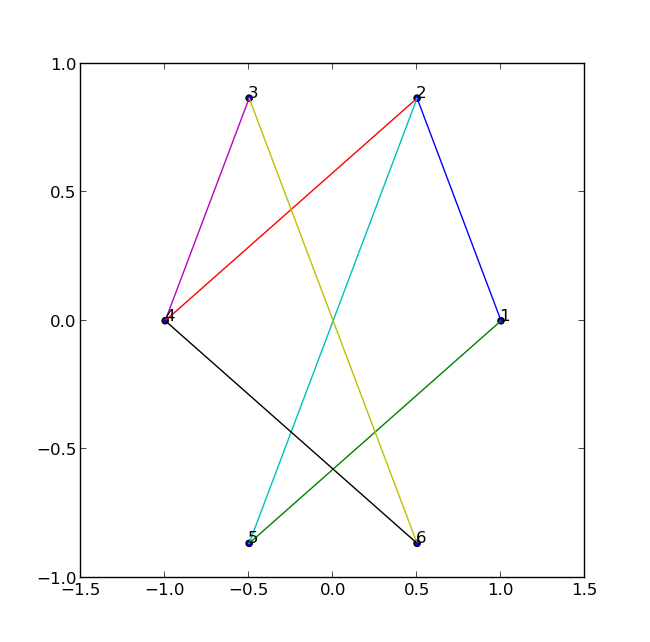
\includegraphics[width=1.\textwidth]{ex1p0}\\
			\end{minipage}\hfill
			\begin{minipage}[b]{.24\textwidth}
			\centering
			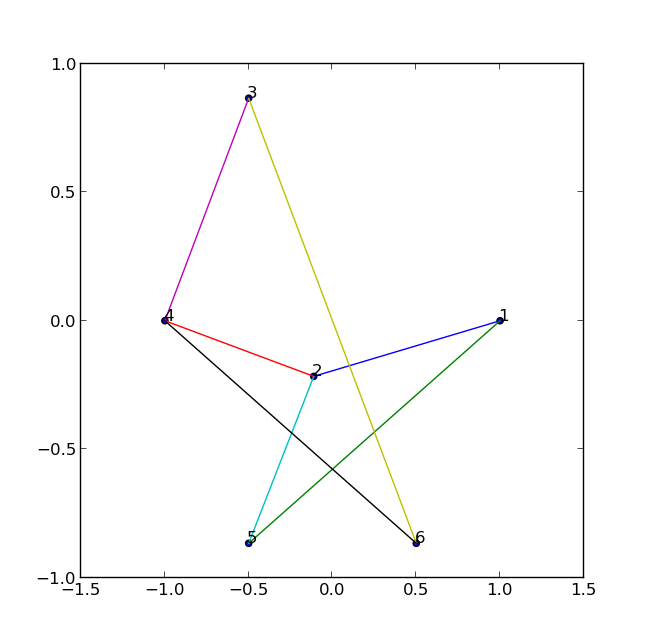
\includegraphics[width=1.\textwidth]{ex1p1}\\
			\end{minipage}
			\begin{minipage}[b]{.24\textwidth}
			\centering
			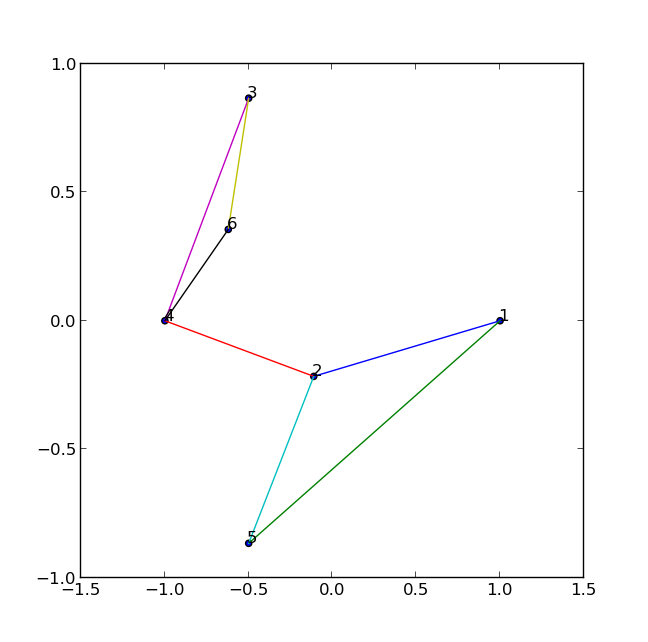
\includegraphics[width=1.\textwidth]{ex1p2}\\
			\end{minipage}\hfill
			\begin{minipage}[b]{.24\textwidth}
			\centering
			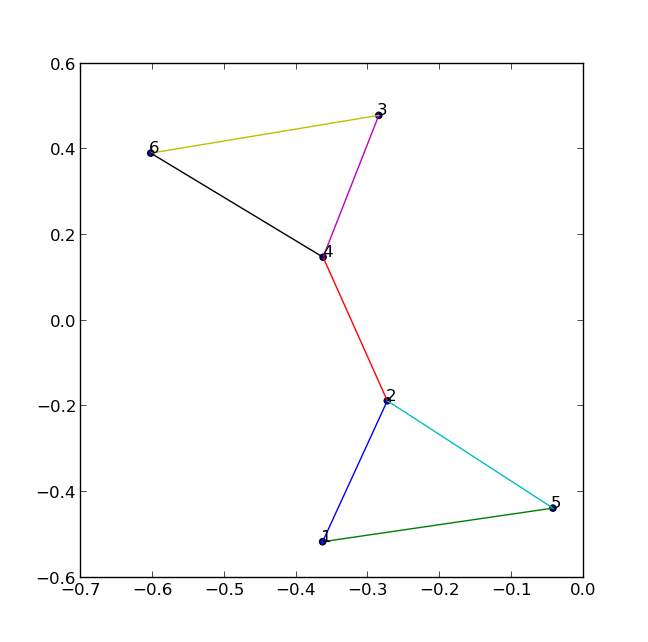
\includegraphics[width=1.\textwidth]{ex1p49}\\
			\end{minipage}\hfill

		\caption{Drawing of a small graph in 4 different states, compare Fig.2 in \cite{TomihisaKamada1989}}\label{fig: 1}
\end{figure}


Our results with KKA can be seen in the following table. Run time on an  Intel Core i3-2310M CPU @ 2.10GHz $\times$ 4 . Parameter $K=1, \ L_0 = 1, \ \epsilon = 0.001$.
\begin{table}

\begin{tabular}{|c|c||c|c|c|c|}
\hline
Algorithm: & & \multicolumn{2}{|c|}{Kamda Kawai} &  \multicolumn{2}{|c|}{Multi Scale}  \\
\hline
\hline 
Graph & $|V|$ & Time & Iterations & Time & Iterations\\ 
\hline
Small Graph & 6 & 0.169s & 47 &- & -\\ 
\hline 
Pyramid Graph & 10 & 0.370s & 45 &0.269s & 1 \\ 
\hline 
Non Symmetric Graph & 10 & FC & FC & 0.279s & 1\\ 
\hline 
Binary Graph(3) & 7 & 0.136s & 30 & -&-\\ 
\hline 
Binary Graph (4) & 15 & 1.97s & 131 & 0.373s& 1 \\ 
\hline 
Binary Graph (5) & 31 & 17.745s & 323 &7.021915s & 2 \\ 
\hline  & a & a & a	& & \\ 
\hline 
\end{tabular} 
\end{table}
The Non Symmetric graph reaches the maximum number of iterations (FC failed to converge). But the drawing can be seen as good. For these small graphs, the multi scale algorithm is very fast, but it also doesn't reach acceptable drawings for our standard parametrisation.


\FloatBarrier 
\subsubsection*{Algorithm of Harel and Koren}

Comparing with the Algorithm of Kamada and Kawai the algorithm of Harel and Koren includes 4 parameters: minimal size of the coarsest graph ($\it MinSize$), ratio between number of vertices in two consecutive levels ($Ratio$), number of iterations of local beautification ($Iterations$), size of the neighbourhood ($Rad$) (as further parameter one can consider the desired length of graph edges ($L$), but author do not mention it specially). The authors claim, that for all examples in paper they used following parameters: $MinSize=10$, $Ratio=3$, $Iterations=4$, $Rad = 7$ (for complete binary tree $Rad$ was set to $16$ or $17$) and achieved reasonable results.

Unfortunately, it was not always the case in our evaluation. So on figure \ref{fig: difMinSize} one can see that in case of square grid graphs some vertices stay clustered after final iteration of the algorithm with the default settings. On the other hand, in case of complete binary tree default setting deliver better drawing results (compare \ref{fig: btrees}).

\begin{figure}[htb]
	 \begin{subfigure}{0.5\textwidth}
		   \centering
           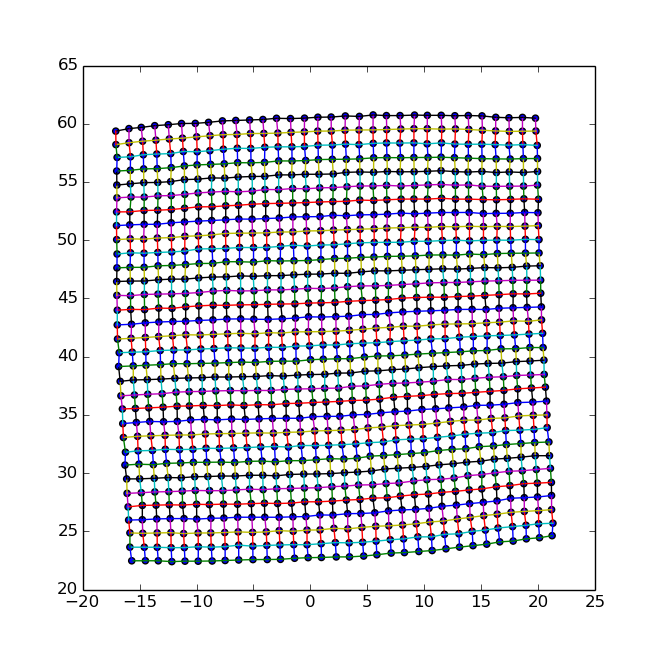
\includegraphics[scale=0.45]{results_Harel/HK_grid32x32_m2r2.png}
           \caption{$MinSize=2$, $Ratio=2$}
     \end{subfigure}
	 \begin{subfigure}{0.5\textwidth}
			\centering
           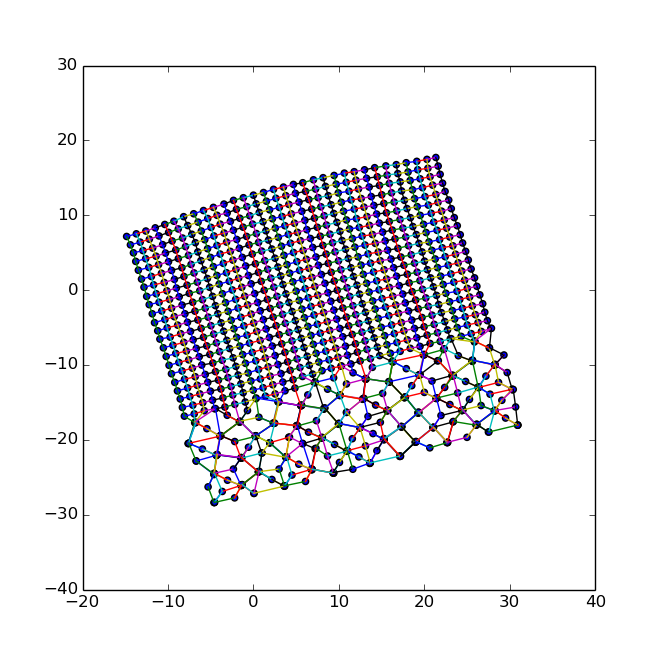
\includegraphics[scale=0.45]{results_Harel/HK_grid32x32_m10_r3.png}
            \caption{$MinSize=10$, $Ratio=3$}
     \end{subfigure}
     \caption{Square grid graph $32\times 32$ (compare figure $1$ in \cite{DavidHarel2002})}
     \label{fig: difMinSize}
\end{figure}     

\begin{figure}[htb]
	 \begin{subfigure}{0.5\textwidth}
		   \centering
           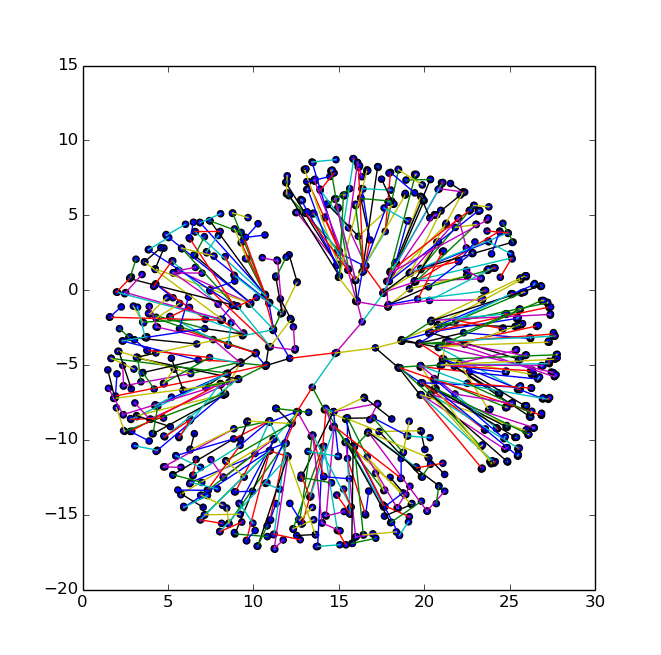
\includegraphics[scale=0.45]{results_Harel/HK_btree1023_m2_r2_rad18.png}
           \caption{$MinSize=2$, $Ratio=2$, $Rad =18$}
     \end{subfigure}
	 \begin{subfigure}{0.5\textwidth}
			\centering
           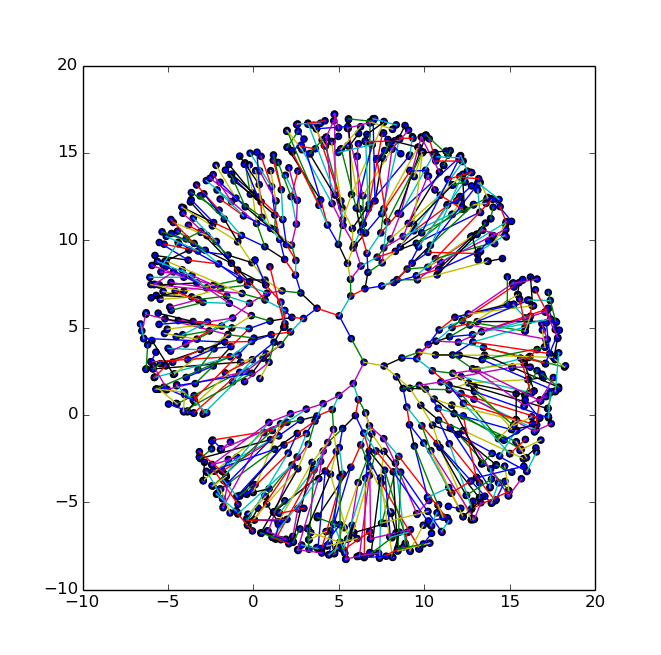
\includegraphics[scale=0.45]{results_Harel/HK_btree1023_m10_r3_rad18.png}
            \caption{$MinSize=10$, $Ratio=3$, $Rad =18$}
     \end{subfigure}
     \caption{Complete binary tree with $1023$ vertices (compare figure $6$ in \cite{DavidHarel2002})}
     \label{fig: btrees}
\end{figure}     

\FloatBarrier 

We also find out, that a random noise added to vertex coordinates (see line $10$ in algorithm \ref{HK}) has some impact on the end result. On the fig. \ref{fig: compareRand} one can see that adding smaller noise ( for example from $(0,0)$ to $(0.1, 0.1)$) leads to better drawing result in our implementation.


\begin{figure}
\begin{minipage}[0.2\textheight]{\textwidth}	%step3
	 \begin{subfigure}{0.5\textwidth}
		   \centering
           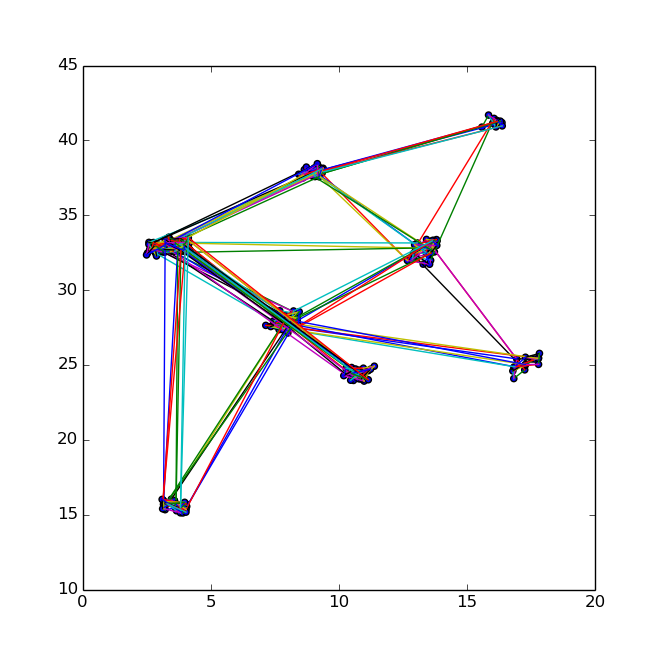
\includegraphics[scale=0.4]{results_Harel/rand1/HK_step3_eps1.png}
           \caption{Step $3$}
     \end{subfigure}
	 \begin{subfigure}{0.5\textwidth}
			\centering
            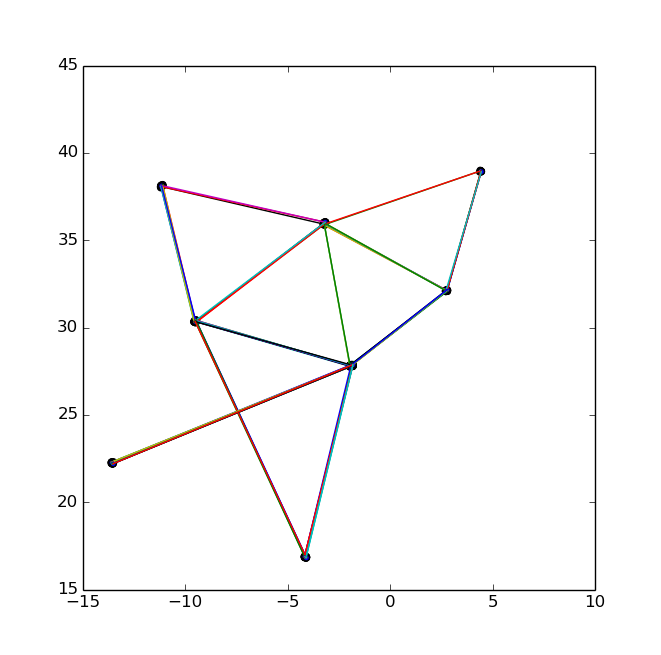
\includegraphics[scale=0.4]{results_Harel/rand01/HK_step3_eps01.png}
            \caption{Step $3$}
     \end{subfigure}        
\end{minipage}

\begin{minipage}[0.2\textheight]{\textwidth}	%step5
	 \begin{subfigure}{0.5\textwidth}
		   \centering
           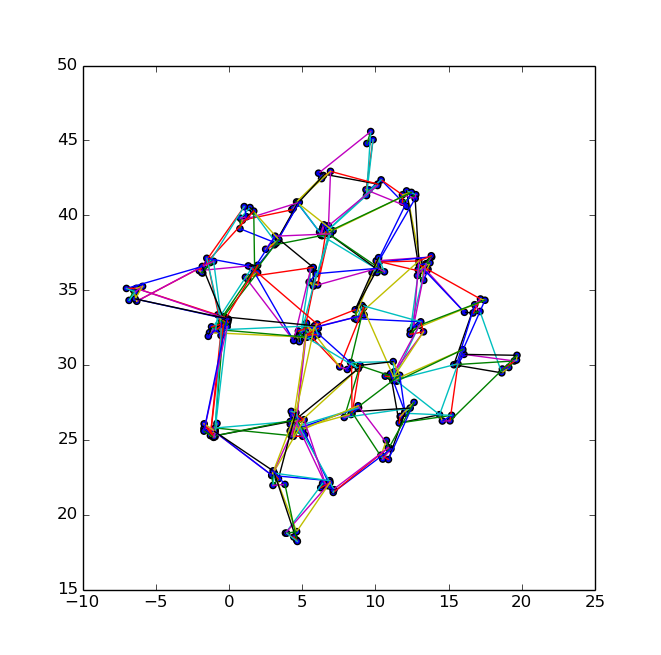
\includegraphics[scale=0.4]{results_Harel/rand1/HK_step5_eps1.png}
           \caption{Step $5$}
     \end{subfigure}
	 \begin{subfigure}{0.5\textwidth}
	 			\centering
            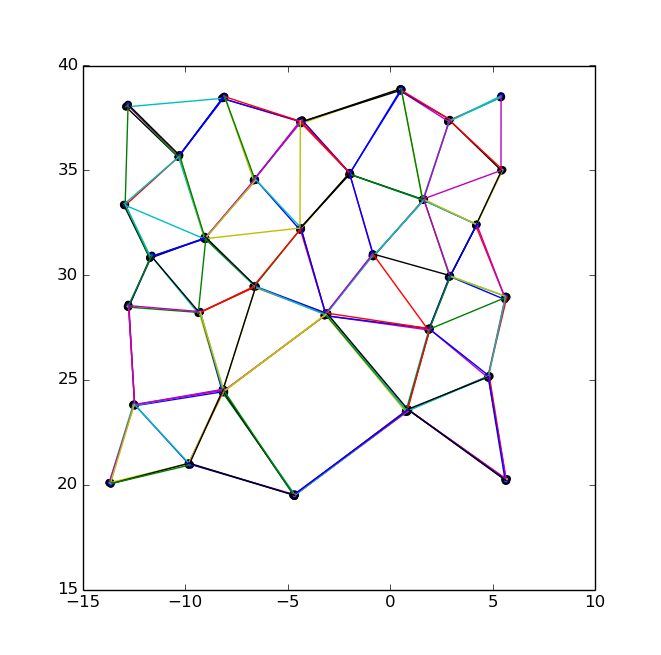
\includegraphics[scale=0.4]{results_Harel/rand01/HK_step5_eps01.png}
            \caption{Step $5$}
     \end{subfigure}        
\end{minipage}
\begin{minipage}[0.2\textheight]{\textwidth}	%step8
	 \begin{subfigure}{0.5\textwidth}
		   \centering
           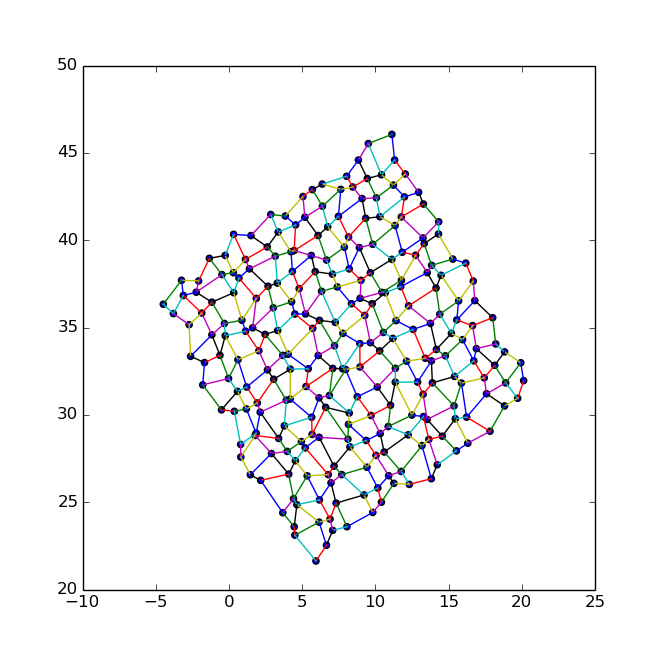
\includegraphics[scale=0.4]{results_Harel/rand1/HK_step8_eps1.png}
           \caption{Step $8$}
     \end{subfigure}
	 \begin{subfigure}{0.5\textwidth}
	 	    \centering
            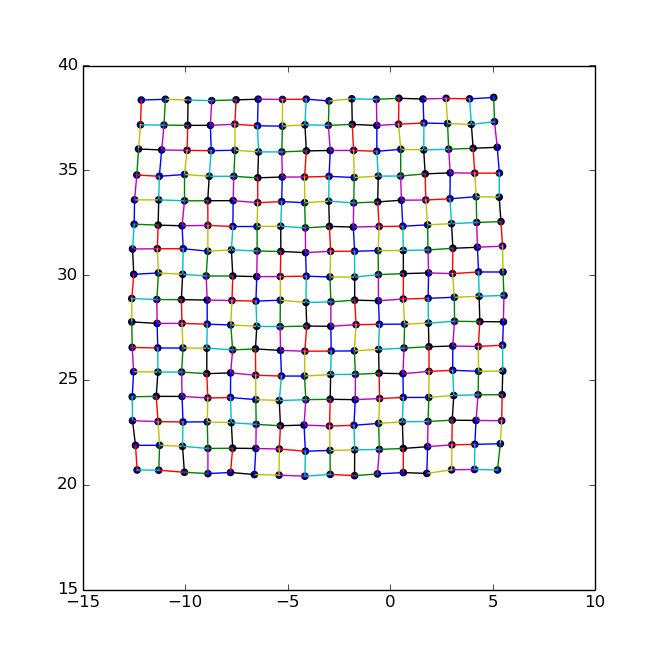
\includegraphics[scale=0.4]{results_Harel/rand01/HK_step8_eps01.png}
            \caption{Step $8$}
     \end{subfigure}        
\end{minipage}

\caption{Influence of the random noise added to coordinates of vertices on the example of grid graph $16\times16$. Left column : $(0,0)<rand<(1,1)$, right column - $(0,0)<rand<(0.1,0.1)$}
\label{fig: compareRand}
\end{figure}	

\FloatBarrier

On the figure \ref{fig: sgrid} we show the result of applying the HKA to the sparse grid graphs ($1/3$ of edges were omitted). Unfortunately, the images do not look so spectacular as in original paper (see figure $4$ in \cite{DavidHarel2002}).
\begin{figure}[htb]
	 \begin{subfigure}{0.5\textwidth}
		   \centering
           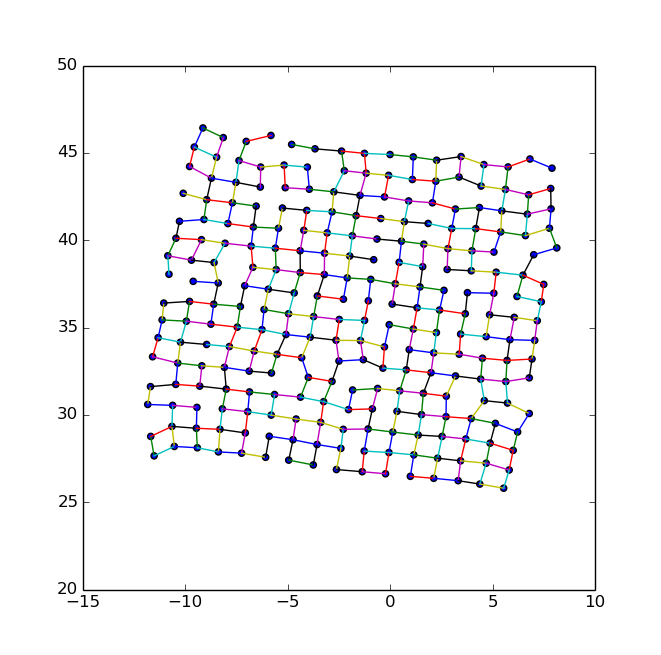
\includegraphics[scale=0.45]{results_Harel/HK_sgrid16x16_m2r2.png}
           \caption{Sparse square grid graph $16\times 16$ ($256$ vertices), $MinSize=2$, $Ratio=2$}
     \end{subfigure}
	 \begin{subfigure}{0.5\textwidth}
			\centering
           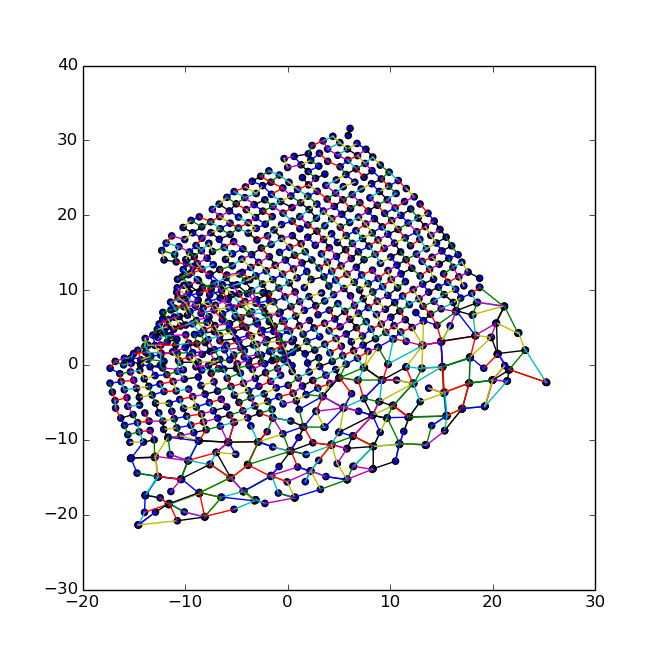
\includegraphics[scale=0.45]{results_Harel/HK_sgrid32x32_m10_r3.png}
            \caption{Sparse square grid graph $32\times 32$ ($1024$ vertices), $MinSize=10$, $Ratio=3$}
     \end{subfigure}
     \label{fig: sgrid}
\end{figure}     

\newpage

The performance of our implementation of HKA can be seen in the table below. Computations were maid on an Intel Core i7-3520M CPU @ 2.90GHz.

\begin{table}[htb]

\begin{tabular}{|c|c||c|c|c|c|c|}
\hline
Algorithm: & & \multicolumn{2}{|c|}{Kamda Kawai} &  \multicolumn{2}{|c|}{Multi Scale} & Parameters \\
\hline
\hline 
Complete Binary Graph & 255  & & & $0.626503$s    & $3$ & $MinSize=10$, $Ratio=3$, $Rad = 18$\\ 
\hline 
Complete Binary Graph & 1023 & & & $1402.674150$s & $5$ & $MinSize=10$, $Ratio=3$,$Rad = 18$\\ 
\hline 
Complete Binary Graph & 1023 & & & $??????$s & $9$ & $MinSize=2$, $Ratio=2$, $Rad = 18$\\ 
\hline \hline
Square Grid Graph     & 256 & & & $20.029714$s & $8$ & $MinSize=2$, $Ratio=2$\\ 
\hline
Square Grid Graph     & 256 & & & $0.615102$s & $3$ & $MinSize=10$, $Ratio=3$\\ 
\hline
Square Grid Graph     & 1024 & & & $3854.181407$s & $10$ & $MinSize=2$, $Ratio=2$\\ 
\hline
Square Grid Graph     & 1024 & & & $1403.437832$s & $5$ & $MinSize=10$, $Ratio=3$\\ 
\hline\hline
Sparse Square Grid Graph & 256 & & & $20.168194$s & $8$ & $MinSize=2$, $Ratio=2$\\ 
\hline
Sparse Square Grid Graph & 1024 & & & $1439.099359$s & $5$ & $MinSize=10$, $Ratio=3$\\ 

\hline 
\end{tabular} 
\end{table}
\FloatBarrier 

\section{Conclusions}

\bibliography{literatur}
\bibliographystyle{siam}

\end{document}